
\subsection{Residual}
\label{sec:residual}

\paragraph{Motivation.}
\label{sec:residual-motivation}
% Background: the residual stream is the only path that carries information across depth
Residual connections give every block a direct path to the network output~\citep{he2016resnet}. 
Pre-normalization keeps training stable at scale~\citep{xiong2020layernorm}, but it attenuates the signal each layer receives: every block reads the same stream, so a feature written early must compete with everything written after it. 
Several lines of work address this by adding paths that bypass the bottleneck, including dense inter-layer connectivity~\citep{huang2017densenet}, an extra residual path for attention values~\citep{zhou2024valueresidual}, and cross-layer reuse of cached states~\citep{sun2024yoco}.

Work that modifies the residual path directly falls into two families. 
The first makes each layer's read and write more expressive, following highway networks~\citep{srivastava2015highway}. 
The second widens the stream itself: Alternating Updates (AltUp)~\citep{baykal2023altup} and Hyper-Connections (HC)~\citep{zhu2024hyper} replace the single residual vector with several parallel branches. 
The two are complementary: widening adds capacity, and a richer read/write mechanism decides how that capacity is spent.

\paragraph{Widening the Residual Stream.}
\label{sec:residual-width}
% The cheapest possible widening
We first study how much of the reported gain comes from width alone, using a
simplified variant of AltUp~\citep{baykal2023altup} that fits a pre-norm
network. The residual state before block $\ell$ is a set of $n_r$ branches
$\bm{R}^{(\ell)}\in\mathbb{R}^{n_r\times d}$, where $d$ is the hidden size
and $\bm{R}^{(\ell)}_i$ denotes branch $i$. Each block holds $n_r$ learnable
scalars $\bm{h}\in\mathbb{R}^{n_r}$ and reads its input as a weighted sum of
the branches,
\begin{equation}
\bm{x}^{(\ell)} = \sum_{i=1}^{n_r} h_i\,\bm{R}^{(\ell)}_i .
\label{eq:altup-read}
\end{equation}
The block output $\bm{y}^{(\ell)}$ is then written back to a single branch,
chosen round-robin by depth:
\begin{equation}
\bm{R}^{(\ell+1)}_i =
\bm{R}^{(\ell)}_i + \mathbf{1}\left[i = \ell \bmod n_r\right]\bm{y}^{(\ell)} .
\label{eq:altup-write}
\end{equation}
This adds $n_r$ parameters per block and no matrix multiplication, so its
compute cost is negligible; the extra cost is the memory traffic of carrying
$n_r$ branches instead of one. Even so, it lowers the training loss of a
25B-A3B MoE model trained on 400B tokens by roughly $0.01$. Widening alone
therefore yields a substantial loss reduction. The question that remains is
how much read/write machinery is worth adding on top of the widened stream to
reach a good balance of performance, efficiency, and stability.

\paragraph{Hyper-Connections (HC).}
\label{sec:residual-hc}
% General form
HC generalizes Eq.~\eqref{eq:altup-read} and Eq.~\eqref{eq:altup-write} into three learnable operators.
A read operator $\bm{H}_{\mathrm{mix}}$ forms the block input, a write operator $\bm{H}_{\mathrm{combine}}$ distributes the block output over branches, and a mixing operator $\bm{H}_{\mathrm{res}}$ exchanges information between branches:
\begin{align}
\bm{x}^{(\ell)} &= \bm{H}_{\mathrm{mix}}^{\top}\bm{R}^{(\ell)}, \label{eq:hc-mix}\\
\bm{y}^{(\ell)} &= \mathcal{F}^{(\ell)}\left(\operatorname{Norm}\left(\bm{x}^{(\ell)}\right)\right), \label{eq:hc-block}\\
\bm{R}^{(\ell+1)} &= \bm{H}_{\mathrm{res}}\,\bm{R}^{(\ell)}
   + \bm{H}_{\mathrm{combine}}\,\bm{y}^{(\ell)\top}, \label{eq:hc-combine}
\end{align}
with $\bm{H}_{\mathrm{mix}},\bm{H}_{\mathrm{combine}}\in\mathbb{R}^{n_r}$ and $\bm{H}_{\mathrm{res}}\in\mathbb{R}^{n_r\times n_r}$. In the notation of HC these are $\bm{A}_m$, $\bm{B}$ and $\bm{A}_r$.
% Where the three operators come from
The three operators are predicted from the residual state. Let $\overline{\bm{R}}=\operatorname{norm}(\bm{R}^{(\ell)})$ be a normalized view of the branches. Each operator is then the sum of a static term and a data-dependent term:
\begin{align}
\bm{H}_{\mathrm{mix}} &= \bm{H}^{\mathrm{s}}_{\mathrm{mix}}
   + \bm{\lambda}_{m}\odot\phi\left(\overline{\bm{R}}\,\bm{W}_{m}\right),
   \label{eq:hc-param-mix}\\
\bm{H}_{\mathrm{combine}} &= \bm{H}^{\mathrm{s}}_{\mathrm{combine}}
   + \bm{\lambda}_{c}\odot\phi\left(\overline{\bm{R}}\,\bm{W}_{c}\right),
   \label{eq:hc-param-combine}\\
\bm{H}_{\mathrm{res}} &= \bm{H}^{\mathrm{s}}_{\mathrm{res}}
   + \bm{\lambda}_{r}\odot\phi\left(\overline{\bm{R}}\,\bm{W}_{r}\right),
   \label{eq:hc-param-res}
\end{align}
where $\bm{H}^{\mathrm{s}}_{\star}$ is a learnable static term, $\bm{W}_{\star}$ projects the normalized residual, $\phi$ is an activation function, and $\bm{\lambda}_{\star}$ is a learnable scale, with $\star$ standing for any of the three operators. HC uses $\phi=\tanh$ with $\bm{\lambda}_{\star}$ initialized to $0.01$; mHC~\citep{xie2025mhc} uses a sigmoid and additionally constrains $\bm{H}_{\mathrm{res}}$ to a manifold of doubly stochastic matrices.
% Initialization and the static special case
Specifically, we set the static terms to $\bm{H}^{\mathrm{s}}_{\mathrm{mix}} = \bm{e}_{\ell\bmod n_r}$, $\bm{H}^{\mathrm{s}}_{\mathrm{combine}} = \bm{1}$, and $\bm{H}^{\mathrm{s}}_{\mathrm{res}} = \bm{I}$. With $\bm{W}_{\star}=\bm{0}$, this initialization starts the widened network exactly at the pre-norm baseline; with $\bm{\lambda}_{\star}=\bm{0}$ throughout, the operators stay static and the widened stream costs no extra computation, which recovers the simplified AltUp variant above.

\paragraph{Design Ablation.}
\label{sec:residual-ablation}
Starting from the static operators, we kept the added expressiveness only where
it paid for itself.
Tab.~\ref{tab:residual-ablation} reports the endpoints of that progression,
evaluated with the benchmark suite and evaluation pipeline of
\S\ref{sec:gdn-ablation}. Five observations shaped the final design.
\begin{itemize}[leftmargin=1.5em]
\item \textbf{Bounded positive gates.} A sigmoid gate is better than $\tanh$
  in both loss and training stability. This agrees with
  mHC~\citep{xie2025mhc} and is consistent with the observation in the GDN
  and attention components that sigmoid gates outperform SiLU or $\tanh$.
\item \textbf{Data dependence.} Making $\bm{H}_{\mathrm{mix}}$ and $\bm{H}_{\mathrm{combine}}$ data-dependent reduces loss by 0.002 over the static variant, whereas the static variant reduced loss by 0.021 over the pre-norm baseline. 
The benchmark gain reverses this ratio: 1.98 points from static to dynamic against 1.58 from baseline to static (Tab.~\ref{tab:residual-ablation}).  
This is one of several places in this report where loss and downstream accuracy do not move together.
\item \textbf{Read granularity matters more than write granularity.} Refining
  $\bm{H}_{\mathrm{mix}}$ in Eq.~\eqref{eq:hc-mix} from one scalar per branch
  to one weight per branch and channel helps. The same refinement of
  $\bm{H}_{\mathrm{combine}}$ in Eq.~\eqref{eq:hc-combine} gives almost
  nothing, so the write stays a per-branch scalar.
\item \textbf{Read all branches.} Predicting the operators from all branches
  is better than using only the last branch or pooling the branches first.
  Normalizing each branch separately, that is, a group RMSNorm over the
  widened stream, gives a further gain.
\item \textbf{$\bm{H}_{\mathrm{res}}$ adds little.} Once the read and the
  write are expressive enough, adding the $n_r\times n_r$ mixing operator
  brings no significant improvement.
\end{itemize}

\begin{table*}[t]
\centering
\small
\setlength{\tabcolsep}{3.5pt}
\caption{Residual read/write ablation on 25B-A3B MoE models
 trained on 560B tokens. The benchmarks and the evaluation pipeline are those
 of \S\ref{sec:gdn-ablation}. All widened variants use $n_r=4$ branches;
 \emph{static} is the case $\bm{\lambda}_{\star}=\bm{0}$ of
 Eq.~\eqref{eq:hc-param-mix}--\eqref{eq:hc-param-res}, \emph{dynamic} its
 data-dependent counterpart.}
\label{tab:residual-ablation}
\resizebox{\textwidth}{!}{%
\begin{tabular}{lrrrrrrrrrrr}
\toprule
& & \multicolumn{3}{c}{Knowledge} & \multicolumn{2}{c}{STEM} & Reasoning
  & Multilingual & \multicolumn{2}{c}{Code} & \\
\cmidrule(lr){3-5} \cmidrule(lr){6-7} \cmidrule(lr){8-8}
  \cmidrule(lr){9-9} \cmidrule(lr){10-11}
Residual & Loss & MMLU & MMLU-Pro & SuperGPQA & MATH & GSM8K & BBH & MMMLU
  & EvalPlus & MultiPL-E & Avg. \\
\midrule
Pre-norm
& 1.617 & 64.29 & 38.40 & 21.78 & 53.92 & 77.41 & 64.73 & 51.26 & 49.25
  & 37.15 & 50.91 \\
mHC (static)
& 1.596 & 64.62 & 43.69 & 22.20 & 55.08 & 78.05 & 65.42 & 52.78 & 49.59
  & 40.94 & 52.49 \\
mHC (dynamic)
& 1.594 & 66.11 & 45.84 & \textbf{24.20} & 59.54 & \textbf{78.51} & 66.01
  & \textbf{56.61} & \textbf{52.16} & 41.30 & 54.47 \\
GR
& 1.590 & \textbf{66.69} & \textbf{46.02} & 23.80 & \textbf{61.18} & 78.20
  & \textbf{66.54} & 56.19 & 51.36 & \textbf{42.00} & \textbf{54.66} \\
\bottomrule
\end{tabular}
}
\end{table*}

Widening the stream with static operators is already worth $1.58$ points of average accuracy over the pre-norm baseline, and making the read and the
write data-dependent adds a further $1.98$. The loss gap between mHC static and dynamic is only $0.002$, yet the benchmark gap is substantial; this is a case where loss alone would have understated the value of the change,
and it reinforced our practice of checking benchmarks alongside loss
throughout the design process. We describe the concrete design of GR below.

\paragraph{Gated Residual.}
\label{sec:residual-gr}
In separate work~\citep{qiu2026unified}, we had found that adding a lightweight elementwise self-gate
after RMSNorm, which we call GatedNorm, markedly improves training stability:
\begin{equation}
\operatorname{GatedNorm}(\bm{u}) = \operatorname{RMSNorm}(\bm{u})\odot
\sigma\left(\bm{W}_{2}\operatorname{SiLU}\left(\bm{W}_{1}
\operatorname{RMSNorm}(\bm{u})\right)\right),
\label{eq:gatednorm}
\end{equation}
where $\bm{W}_1$ and $\bm{W}_2$ form a low-rank bottleneck.
The read the ablation arrives at, elementwise and data-dependent with a
sigmoid gate, is exactly Eq.~\eqref{eq:gatednorm} applied to the widened
stream. We therefore merge the two into a single operator and call the result
Gated Residual (GR).

GR first normalizes each branch independently,
\begin{equation}
\widehat{\bm{R}}_i = \operatorname{RMSNorm}\left(\bm{R}_i;\bm{\gamma}_i\right),
\qquad i=1,\dots,n_r,
\label{eq:gr-norm}
\end{equation}
each with its own gain $\bm{\gamma}_i\in\mathbb{R}^{d}$. It then predicts 
elementwise gating scores per branch and channel from all branches, and averages the gated
branches into the block input:
\begin{align}
\bm{G} &= \operatorname{unvec}\,\sigma\left(\bm{W}_{u}
\operatorname{SiLU}\left(
   \tfrac{1}{n_r}\bm{W}_{d}\operatorname{vec}(\widehat{\bm{R}})\right)\right)
   \in\mathbb{R}^{n_r\times d},
   \label{eq:gr-gate}\\
\bm{x} &= \frac{1}{n_r}\sum_{i=1}^{n_r}\bm{G}_i\odot\widehat{\bm{R}}_i ,
   \label{eq:gr-read}
\end{align}
where $\operatorname{vec}$ stacks the branches into one vector of length
$n_r d$ and $\operatorname{unvec}$ is its inverse, with
$\bm{W}_{d}\in\mathbb{R}^{r\times n_r d}$ and
$\bm{W}_{u}\in\mathbb{R}^{n_r d\times r}$ for a bottleneck rank $r = d / 8$.
The block output $\bm{y}=\mathcal{F}(\bm{x})$ is written to every branch
through one data-dependent scalar per branch:
\begin{align}
\bm{s} &= 2\,\sigma\left(\tfrac{1}{n_r}\bm{W}_{w}
\operatorname{vec}(\widehat{\bm{R}})\right)
   \in\mathbb{R}^{n_r},
   \label{eq:gr-write-gate}\\
\bm{R}'_i &= \bm{R}_i + s_i\,\bm{y} ,
   \label{eq:gr-write}
\end{align}
with $\bm{W}_{w}\in\mathbb{R}^{n_r\times n_r d}$.
Eq.~\eqref{eq:gr-gate} and Eq.~\eqref{eq:gr-write-gate} are the read and
write operators of Eq.~\eqref{eq:hc-param-mix} and
Eq.~\eqref{eq:hc-param-combine} with $\phi=\sigma$, an elementwise
$\bm{H}_{\mathrm{mix}}$, a per-branch scalar $\bm{H}_{\mathrm{combine}}$,
and $\overline{\bm{R}}$ the group-RMSNorm of all branches.
The static term $\bm{H}^{\mathrm{s}}_{\star}$ brings no improvement for GR.
With the current configuration, no special initialization of the learnable
weights is needed, and the static term contributes negligibly; standard
random initialization, as used in the backbone, suffices.
We use $n_r=4$ branches, with a separate GR module for the attention block
and the MLP block of every layer.

In Tab.~\ref{tab:residual-ablation}, GR and mHC (dynamic) differ mainly in
the elementwise $\bm{H}_{\mathrm{mix}}$ and the removal of
$\bm{H}_{\mathrm{res}}$; at this scale the two perform comparably. The
efficiency advantage of GR is that removing $\bm{H}_{\mathrm{res}}$
eliminates a full read of the residual state per block, reducing memory
traffic. 
The stability advantage is twofold: GatedNorm itself improves
training stability (analysed in \S\ref{sec:stability}), and dropping $\bm{H}_{\mathrm{res}}$, which requires separate constraints, removes a potential source of instability.

GR belongs to the same family as HC, mHC and VWN~\citep{seed2025vwn}; what
differs is where the extra expressiveness is spent. HC and mHC keep the read
and the write as per-branch scalars and put capacity into
$\bm{H}_{\mathrm{res}}$, which mHC further constrains to be doubly
stochastic. VWN keeps those scalars as well and instead widens the token
embedding, splitting it into many narrow segments; this splitting likewise
pursues finer-grained read and write operations. GR spends its expressiveness
on the read: the gate is elementwise, and $\bm{H}_{\mathrm{res}}$ is dropped
altogether, which the ablation shows costs nothing and which removes a read
of the whole residual state per block, the dominant inference cost of a
widened stream.

Because the read in Eq.~\eqref{eq:gr-read} already normalizes and gates, GR
also replaces the block's pre-normalization rather than sitting in front of it: Eq.~\eqref{eq:hc-block} loses its $\operatorname{Norm}$, and widening adds no normalization layer. 
And with no mixing operator the branches stay separate, since a branch is only ever written by blocks and read through Eq.~\eqref{eq:gr-read}. 
This makes the information flow easy to follow, which we use in the analysis in \S\ref{sec:residual-analysis}.

\paragraph{Comparison with Attention Residual.}
\label{sec:residual-attnres}


\begin{wraptable}{r}{0.48\linewidth}
\centering
\small
\vskip -0.15in
\setlength{\tabcolsep}{4pt}
\caption{Residual designs at $28$ layers, with and without GatedNorm (GN). 
Loss is the final training loss; $S$ is the number of sublayers summed into one Block AttnRes representation. Subscripts give the change from the column on the left.}
\vskip -0.05in
\label{tab:residual-attnres}
\begin{tabular}{lcc}
\toprule
Residual design & Loss & \makecell{Loss + GN} \\
\midrule
Pre-norm residual    & 1.789 & $1.787_{-0.002}$ \\
Block AttnRes, $S=4$ & 1.773 & $1.768_{-0.005}$ \\
Block AttnRes, $S=2$ & 1.770 & $1.766_{-0.004}$ \\
Full AttnRes         & 1.762 & $\mathbf{1.758}_{-0.004}$ \\
GR ($n_r=4$)         & --- & 1.762 \\
\bottomrule
\end{tabular}
\vskip -0.15in
\end{wraptable}

Attention Residual
(AttnRes)~\citep{kimiteam2026attentionresiduals} uses a softmax attention over earlier layers' outputs to determine each sublayer's read. Full AttnRes attends over the output of every preceding sublayer. 
Block AttnRes partitions the $L$
sublayers into blocks of $S$, sums each block into one representation, and attends over those.

Tab.~\ref{tab:residual-attnres} compares both variants against GR in our setting, a $28$-layer model ($L=56$ sublayers), each with and without GN. 
Full AttnRes is the strongest setting of that family and lands level with GR at $1.762$, while summarizing blocks costs $0.008$ at $S=2$ and $0.011$ at $S=4$. 
The same ordering holds deeper: at $48$ layers, Block
AttnRes at $S=4$ reaches $1.711$ against $1.707$ for GR.
GN lowers the loss at every setting, by $0.004$--$0.005$ on AttnRes and by $0.002$ on the plain pre-norm baseline. 
The gate helps more when the input a sublayer reads is more complex, which is the same gate GR carries inside its read.




\paragraph{What the Branches Are Used For.}
\label{sec:residual-analysis}
The ablation shows that GR improves both loss and benchmarks, but what mechanism produces the gain? 
As GR has no residual branch mixing, each branch is
a plain accumulator of past outputs, and we can decompose exactly what each block reads into contributions from every earlier block. 
We use this decomposition to compare a GR model against an otherwise identical reference without GR, and find that the extra width is spent on several specific paths: one branch preserves early attention outputs across many layers, while the other three stay local.

\emph{The statistic.}
Branch $c$ before block $v$ holds
\begin{equation}
\bm{R}^{(v)}_c = \bm{R}^{(0)}_c + \sum_{u<v} s^{(u)}_c\,\bm{y}^{(u)},
\label{eq:gr-accumulator}
\end{equation}
where $\bm{R}^{(0)}_c$ is the initial value of branch $c$ (the token
embedding), $\bm{y}^{(u)}$ is the output of block $u$, and $s^{(u)}_c$ is
the scalar write gate of Eq.~\eqref{eq:gr-write-gate} controlling how much
of $\bm{y}^{(u)}$ enters branch $c$.

Block $v$ reads this branch through the gated read of
Eq.~\eqref{eq:gr-read}: it normalizes the branch, scales it by a learned
per-channel gain $\bm{\gamma}_c$ (from Eq.~\eqref{eq:gr-norm}), gates the
result elementwise with $\bm{G}^{(v)}_c$ (the data-dependent gate of
Eq.~\eqref{eq:gr-gate}), and averages over branches. Since normalization
divides by $\operatorname{rms}(\bm{R}^{(v)}_c)$, the contribution of block
$u$ to block $v$'s input is
\begin{equation}
\bm{a}_{u\to v}
= \frac{1}{n_r}\sum_{c=1}^{n_r}
  \bm{G}^{(v)}_c\odot\bm{\gamma}_c\odot
  \frac{s^{(u)}_c\,\bm{y}^{(u)}}{\operatorname{rms}\left(\bm{R}^{(v)}_c\right)},
\label{eq:gr-attribution}
\end{equation}
evaluated at the gate values the forward pass actually took. Each factor has
a direct reading: $s^{(u)}_c\,\bm{y}^{(u)}$ is what block $u$ deposited on
branch $c$; the division by $\operatorname{rms}(\bm{R}^{(v)}_c)$ accounts
for the normalization applied at read time; $\bm{\gamma}_c$ rescales each
channel; and $\bm{G}^{(v)}_c$ decides how much of this branch block $v$
actually uses.


\begin{figure}[t]
  \centering
  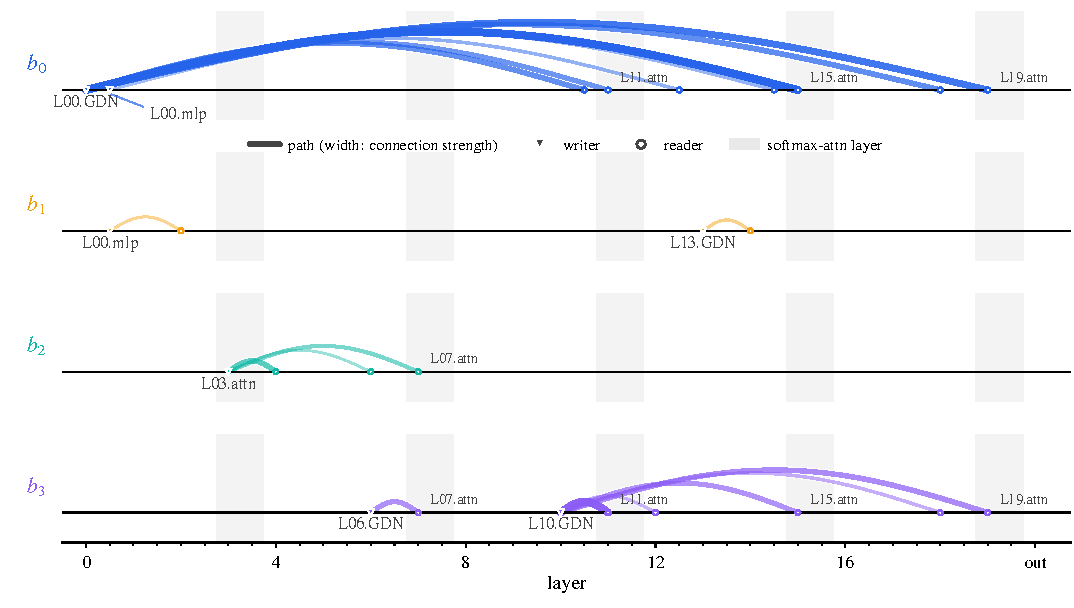
\includegraphics[pagebox=cropbox,width=\linewidth]{figs/paper_gr_excess_paths.pdf}
  \vskip -0.1in
\caption{\textbf{Cross-layer paths added by GR.} Each row corresponds to one residual branch; a connection runs from the sublayer that wrote
into that branch to a later sublayer that reads it back. Vertical position encodes the number of layers skipped; line width and opacity encode $\Delta_{uv}$
(Eq.~\eqref{eq:gr-share}), the additional share of the reader's input supplied by this writer compared to a single residual stream. 
Shaded regions denote softmax-attention layers, every fourth in this hybrid; the rest are GDN, and
sublayers are named accordingly (\texttt{L00.GDN}, \texttt{L03.attn}, \texttt{L00.mlp}). 
Readers are named where they are softmax-attention sublayers, which is where the long-range paths land. 
One branch carries long-range paths (all connections on $b_0$ originate at layer 0 and land past layer 10), while the other
three stay local (median skips of 1.2--3.5 layers). The extra width is spent on a small number of specific paths, mostly preserving early GDN output across depth and
delivering it to the softmax-attention layers. Thresholds and counts are given in the text.}
  \label{fig:gr-excess-paths}
\end{figure}

We report the normalized magnitude of this contribution,
\begin{equation}
\pi_{uv} = \frac{\lVert\bm{a}_{u\to v}\rVert}
                {\sum_{u'<v}\lVert\bm{a}_{u'\to v}\rVert},
\label{eq:gr-share}
\end{equation}
the fraction of block $v$'s input that came from block $u$. Because
Eq.~\eqref{eq:gr-attribution} splits each contribution by branch before
summing, we can see which branch carries each path. The decomposition is
exact: every reader's shares sum to one to within $3\times10^{-8}$.

We compare a 20-layer MoE trained with GR against an otherwise identical reference without GR, same recipe, data, optimizer and training step, probed on the same tokens. 
We report the difference
$\Delta_{uv}=\pi^{\mathrm{GR}}_{uv}-\pi^{\mathrm{ref}}_{uv}$, since
subtracting the reference removes the pattern common to all residual networks,
namely that nearby writers dominate. 


\emph{What the figure shows.}
Fig.~\ref{fig:gr-excess-paths} shows the $21$ paths (out of $780$ ordered
pairs) with $\Delta_{uv}\ge 0.05$ over a skip of at least one layer. To
calibrate: at layer $15$ there are $30$ writers, so an equal split gives
each about $0.03$; a share of $0.13$ is four times that.

One branch carries long-range paths while the other three stay local. Which
branch it is does not matter, since the branches are exchangeable at
initialization, but the pattern is consistent: across five GR checkpoints,
each has exactly one such branch, with a typical skip of $10.9$ layers
against $3.4$--$3.9$ for the rest. Three examples illustrate the pattern;
each gives the share under the reference model (a single residual stream
without GR) and then under GR.
\begin{itemize}[leftmargin=1.5em]
\item Layer $0$ GDN $\to$ layer $15$ attention: the share rises from $0.020$ in the reference to $0.138$ in GR. 
    This share holds at $0.072$--$0.138$ across every reader
  from layer $10$ to $19$ with no downward trend.
  This confirms the outsized role of the first layer in preserving information across depth, consistent with prior observations~\citep{elhage2021mathematical,men2024shortgpt}.
\item Layer $10$ GDN $\to$ layer $11$ attention:
  $\Delta_{uv}=0.117$. The gain is as large as the path above, but over a single layer: GR strengthens short-range connections as well.
\item Layer $0$ MLP, on two branches at once: to layer $15$ on the long-range branch, where its share rises from $0.008$ in the reference no-GR model to $0.058$ in GR; and to layer $2$ on a local one, where it rises from $0.139$ to $0.192$.
The same output reaches a nearby and a distant reader with different strengths, which a single stream cannot express since it has only one decay rate for every writer.
\end{itemize}

The typical long-range path in branch 0 follows from Eq.~\eqref{eq:gr-accumulator}: the branch is written most heavily at layer 0 and barely updated thereafter, so that layer-0 information remain accessible to all subsequent layers.
Furthermore, the sublayers that read most heavily from the GR branches are predominantly the softmax attention layers, indicating that global attention acts as a critical hub for integrating explicit long-range historical context that the GDN layers compress away.

To see the overall pattern, we group all $780$ paths by how many layers they skip and sum $\Delta_{uv}$ within each group, where $\Delta_{uv}$ is the extra share that GR gives to path $(u,v)$ over the reference. 
The result: adjacent-layer paths (skip $1$) collectively gain $0.96$ in share; long-range paths (skip $>12$) collectively gain $0.91$; and mid-range paths
(skip $2$--$12$) collectively lose $3.21$. The weighted-average skip is almost unchanged ($3.97$ vs $3.91$), so the total amount of cross-layer information is similar; what changes is its distribution. 
GR selects a few paths and amplifies them, at the expense of mid-range ones.

\paragraph{Inference Efficiency.}
\label{sec:residual-efficiency}
% GR is memory bound, not compute bound
The inference cost of GR is dominated by the memory traffic of the widened residual state. We therefore looked for ways to move fewer bytes.

The first attempt was to sparsify the read. We observed that in trained models, the write at each GR layer is typically dominated by two branches.
We therefore tried introducing sparse writes, either from scratch or mid-training, where each block reads only the two branches with the highest gate values instead of all $n_r$. 
Pre-training loss and benchmarks were almost unaffected, but the quality degraded clearly after post-training, so we did not adopt it. 
More complex variants, such as varying the sparsity level across layers, did not resolve the issue. 
We note \textit{this as a case where pre-training metrics alone would have led to the wrong decision}. 
Recent work xHC~\citep{zhang2026xhc} explores using a larger $n_r$ to make sparse branch updates easier, but given the memory overhead of a larger $n_r$, we did not explore this direction further.

The second attempt was to keep the residual state in FP8. The gates in GR, gated attention, and GDN all bound the magnitude of what is written into the stream, so residual values stay in a narrow range and are well matched to a low-precision format. 
Storing the branches in FP8 halves the bytes moved for the residual state relative to BF16, with almost no loss in quality.
Finally, the read of Eq.~\eqref{eq:gr-norm}--\eqref{eq:gr-read} and the write of Eq.~\eqref{eq:gr-write-gate}--\eqref{eq:gr-write} are each fused into a single kernel, with the group RMSNorm folded into the read, so the
widened stream is traversed once per block in each direction.